

%%%%%%%
%FIGURE
%
\begin{figure}
  \centering
    \includegraphics[width=12cm]{figures/xyz.pdf}
    \caption{Text for caption}
    \label{fig:xyz}
\end{figure}

%example
\begin{figure}
  \centering
    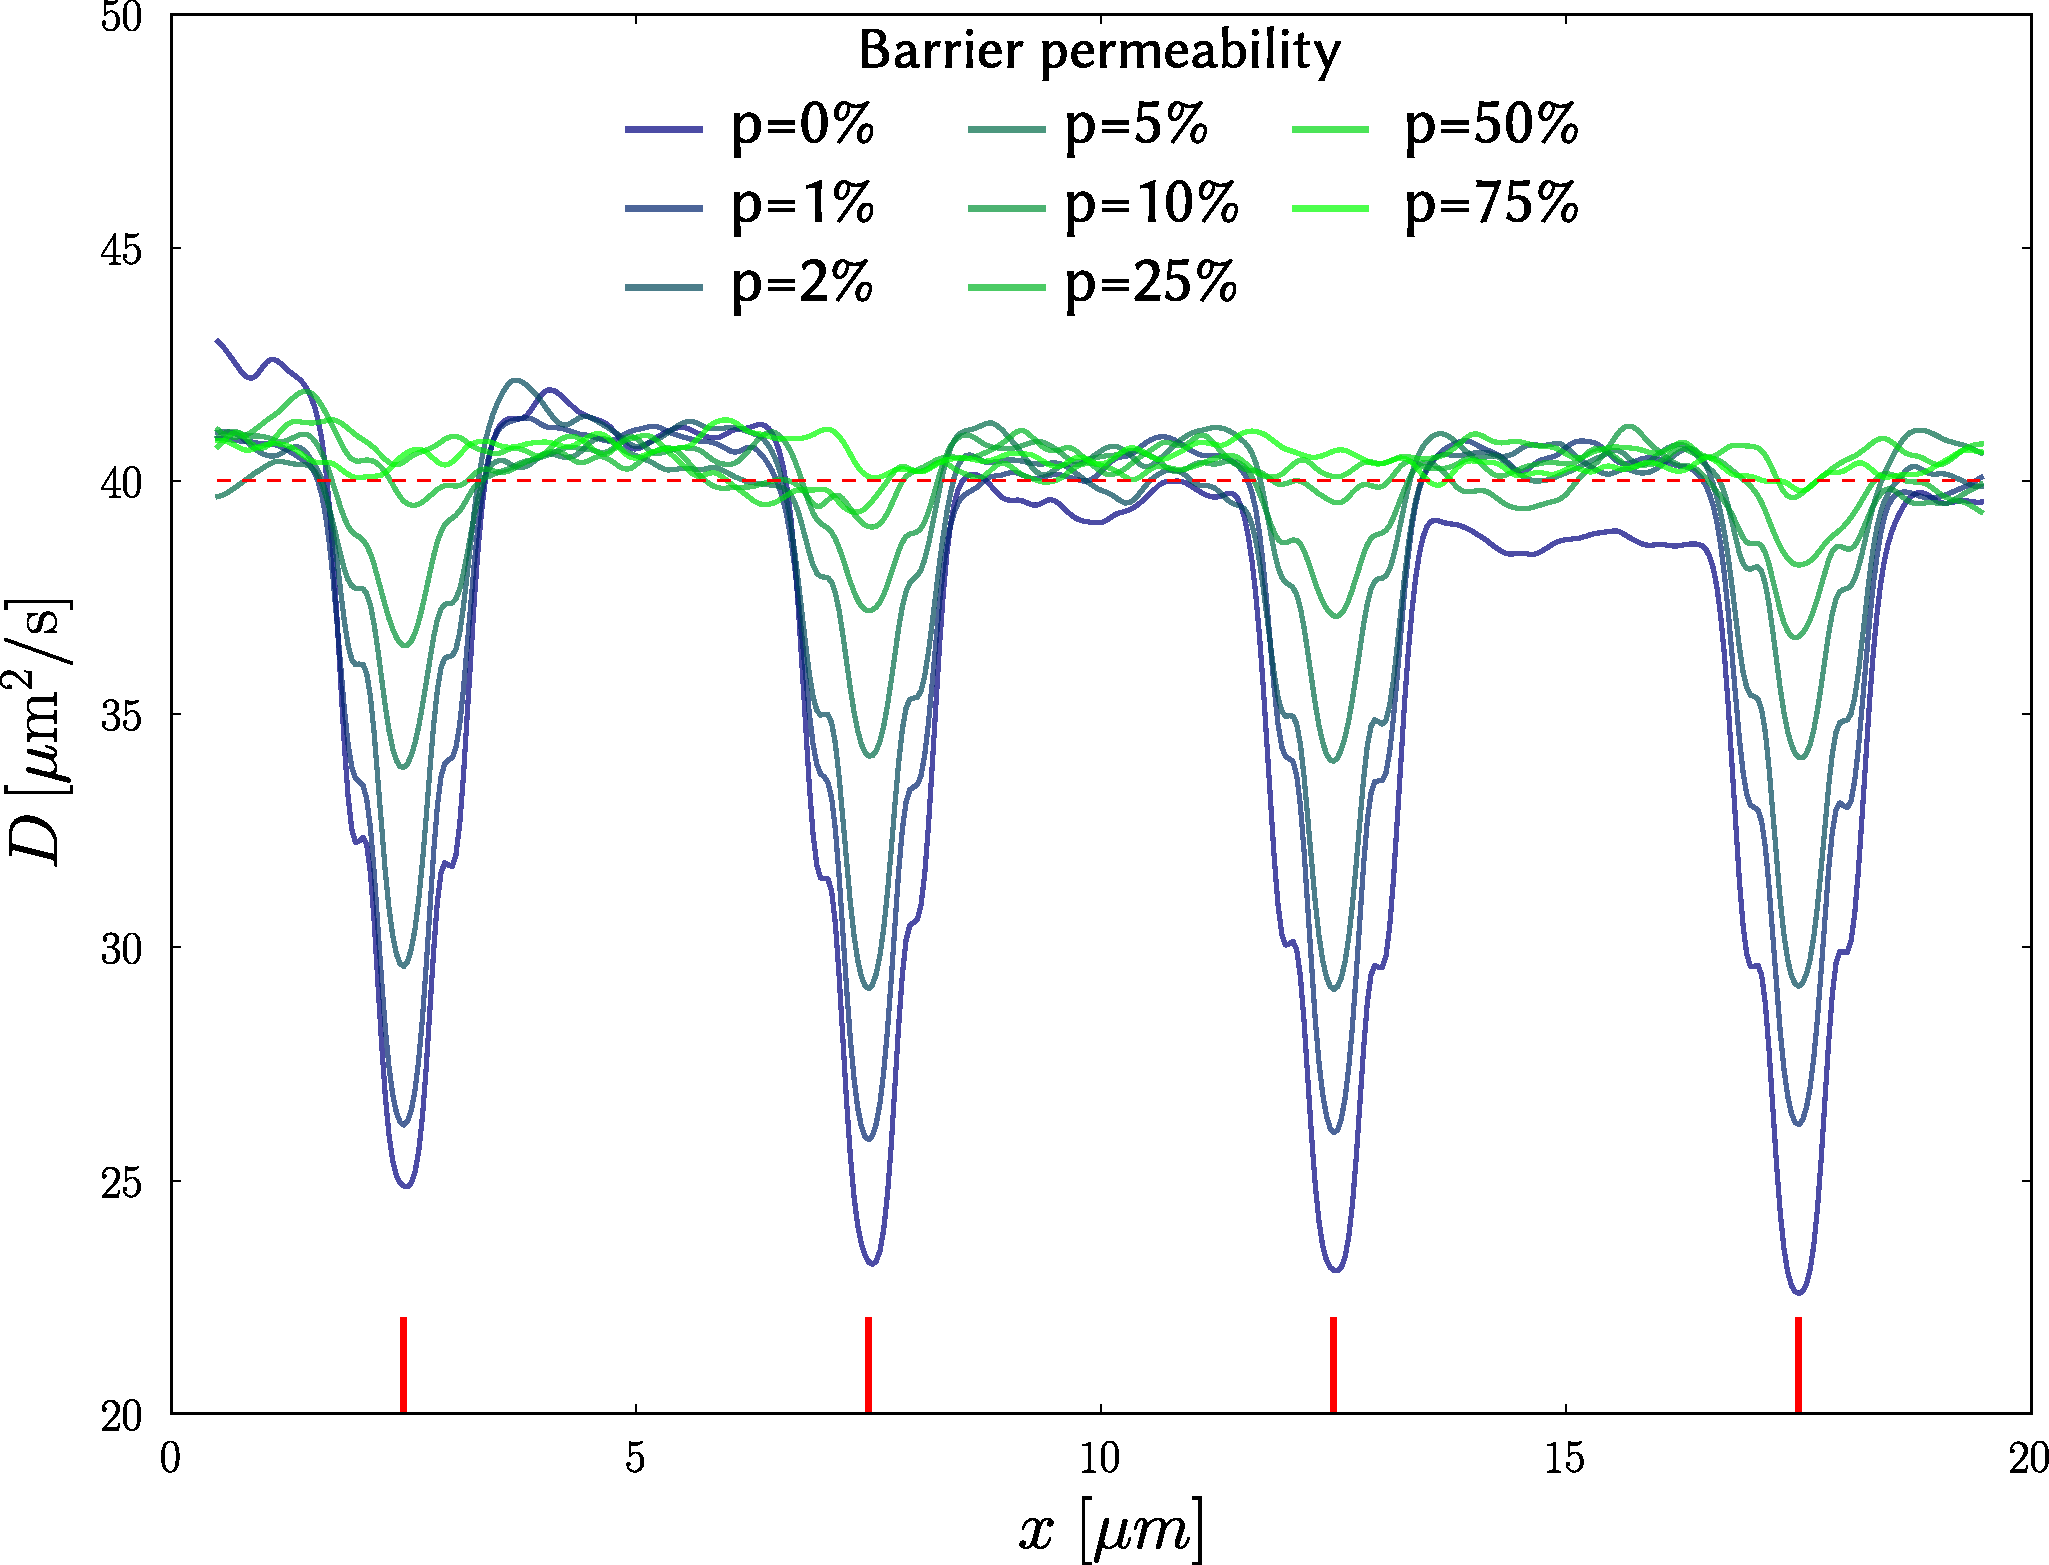
\includegraphics[width=9cm]{figures/range_5.pdf}
    \caption[Regional \acsp{DC} for barriers 5 $\mu$m apart]{\acsp{DC} obtained
    from regional \ac{RICS} analysis of linescan data obtained from a
    computational model. Barriers (indicated by short vertical lines) are
    places 5 $\mu$m apart and their permeability(p) is varied between model
    runs. \acsp{DC} obtained for varying permeability values are shown with
    different lines. The value shown at any $x$ location is the \ac{DC}
    obtained from \ac{RICS} analysis on the 1 $\mu$m segment centered at that
    location.}
    \label{fig:1drange}
\end{figure}

%%%%%%
%TABLE
%
\begin{table}
    \begin{center}
        \input{input/small/xyz}
    \end{center}
    \caption{Text for caption}
    \label{table:xyz}
\end{table}
%Example
\begin{table}
    \begin{center}
        \begin{tabular}{lcccc}

  \hline
  & \multicolumn{4}{c}{Direction} \\
  Model & \multicolumn{2}{c}{transverse} &
  \multicolumn{2}{c}{longitudinal} \\ 
  parameter& \multicolumn{2}{c}{TR (x,z)} & \multicolumn{2}{c}{L (y)} \\
  &min&max&min&max\\
  \hline
  Distance d [$\mu$m] & $0.68\pm 0.10$ & $0.87\pm 0.07$ &
  $0.73\pm 0.13$&$1.02\pm 0.10$ \\
  Pore radius R [nm]  & $7.4 \pm 2.1$ & $30 \pm 8$&
  $6.7\pm 1.8 $&$38\pm 10$\\
  Pore density $\eta$ [$\sfrac{1}{\mu \mathrm{m}^2}$] & $1.2 \pm 0.1$ &
  $29 \pm 23$ & $1.1\pm 0.1$ & $48\pm37$ \\
  $\lambda^{\mathrm{AATP}}$ & $0.78 \pm 0.13$ & $1.0$&$0.78 \pm 0.13$ &$1.0$ \\
  $\lambda^{\mathrm{ADEX}}$ & $0.77 \pm 0.14$ & $1.0$&$0.77 \pm 0.14$ &$1.0$ 
\end{tabular}

    \end{center}
    \caption[Properties of barriers restricting diffusion]{Properties of
    barriers restricting diffusion predicted by stochastic model on the
    basis of RICS measurements. Data presented is mean$\pm$standard
    deviation.}
    \label{table:model_res}
\end{table}
